\section{Vertical Shifts}
The easiest of the transformations to consider is $k$. This variable vertically shifts the function by its value. For example, if $f(x) = x$, then $g(x) = x + 1$, where $k = 1$, is simply the function $f(x)$ but moved up a unit. In the same manner, a function $h(x) = x - 1$, where $k = -1$, is the function $f(x)$ moved down a unit.

\begin{center}
    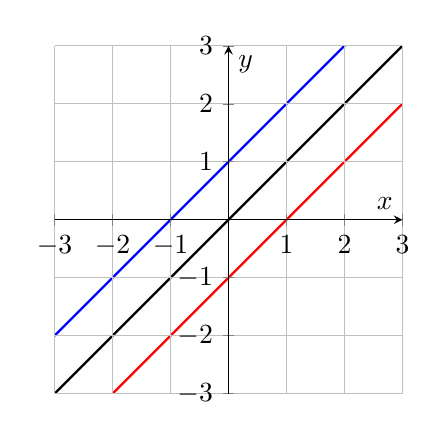
\begin{tikzpicture}
        \begin{axis} [
            axis lines=middle,
            xlabel = $x$, ylabel = {$y$},
            xmin = -3, xmax = 3,
            ymin = -3, ymax = 3,
            xtick distance={1}, ytick distance={1},
            grid = both,
            width = 6cm,
            height = 6cm,
            smooth,
            axis on top
        ]

            \addplot[black, thick, smooth, domain = -3:3, samples = 100]{x};
            \addplot[blue, thick, smooth, domain = -3:3, samples = 100]{x + 1};
            \addplot[red, thick, smooth, domain = -3:3, samples = 100]{x - 1};
        \end{axis}
    \end{tikzpicture}\\
    $f(x) = x$ (Black), 
    $g(x) = x + 1$ (Blue), 
    $h(x) = x - 1$ (Red)
\end{center}
A vertical shift moves all parts of a funtion the specified number of units up or down. That includes asymptotes. For example, if the function I'll redefine as $f(x) = \dfrac{1}{x}$ has a horizontal asymptote of $y = 0$, the new redefined function $g(x) = \dfrac{1}{x} + 1$ wil have a horizontal asymptote of $y = 1$.
\begin{definition}
Given a function $f(x)$ and a vertical shift $k$, the new function $g(x) = f(x) + k$ is the function $f(x)$ vertically translated $k$ units.
\begin{itemize}
    \item When $k < 0$, $f(x)$ moves in the negative $y$ direction (down).
    \item When $k > 0$, $f(x)$ moves in the positive $y$ direction (up).
    \item When $k = 0$, $f(x) = g(x)$. The function does not move.
\end{itemize} 
\end{definition}